\documentclass[../root.tex]{subfiles}

\begin{document}

\section{Rationale}

The idea of constructing a deterministic version of the problem
aims at making it easily solvable with a classic planner such as
Fast Forward or Fast Downward. Two of the most straightforward methods
presented here are those implemented by FF-Replan~\cite{yoon2007ffreplan}:
Single Outcome Determinization and All Outcome Determinization.
However, they make little to no use of the outcome probabilities when
elaborating the deterministic domain. One challenge is to
translate the probability of the outcomes into some feature
of deterministic domains that hints the planner to give
preference to more likely to
succeed plans. The $\alpha$-Cost-Transition-Likelihood~\cite{kaelbling2013integrated}
method that
we will present here does so via translating the transition probabilities
into deterministic costs.
Hindsight
Optimization~\cite{yoon2008probabilistic,yoon2010improving} does so
via outcome
sampling and repeated invocations to a deterministic plan to calculate
an upper bound to the $ Q $ functions (the state-action utility) in the
current state.

However, all the methods presented in this chapter require (or, at the
very least, work more easily) with expanded probability outcomes. We
will elaborate on that in the next Section.

\section{Expansion of probabilistic outcomes}

Typically, probabilistic effects in PPDDL are more easily expressed in
\emph{factored form}. This means that they either nested
(Fig.~\ref{fig:nested-probabilistic}) or put together
in a conjunction (Fig.~\ref{fig:conjunction-probabilistic}).

\begin{figure}[tbhp]
\centering
\begin{subfigure}[b]{0.48\columnwidth}
\begin{lstlisting}[numbers=none]
(and
(probabilistic
0.25 (and
      (forall (?screw - screw)
       (not (fixed-by ?comp ?screw)))
        (forall (?screw - screw
                 ?side_ - side)
        (not (at-side ?screw ?side_)))
      (probabilistic 
        0.5 (loose ?comp)))
0.10 (broken-component ?comp))
(decrease (reward) 1))
\end{lstlisting}
\caption{}
\label{fig:nested-probabilistic}
\end{subfigure}
~
\begin{subfigure}[b]{0.48\columnwidth}
\begin{lstlisting}[numbers=none]
(and
 (probabilistic
  0.25 (and (loose ?comp)
       (when (loose ?comp)
        (removed-non-verified ?comp)))
  0.10 (removed-non-verified ?comp)
  0.12 (broken-component ?comp))
 (probabilistic
  0.12 (broken-tool flat-sd))
 (decrease (reward) 1))
\end{lstlisting}
\caption{}
\label{fig:conjunction-probabilistic}
\end{subfigure}
\caption{
	(a) Nested probabilistic effects. This example is part
	of the effect of the
	\texttt{bash} action of the recycling domain
	(Annex~\ref{chap:ppddl-model}).
	(b) Conjunction of probabilistic effects. This example is part
	of the effect of the \texttt{lever-scara-medium-confidence} of
	the recycling domain (Annex~\ref{chap:ppddl-model}).
}
\label{fig:non-expanded-probabilistic}
\end{figure}

However, all the techniques presented in this chapter are based on
introducing one new action per outcome (except Single-Outcome, which
picks one). Therefore, it is much more convenient to have the
probabilistic effects in expanded form, similarly to
NID rules~\cite{martinez2017relational}.

One could demand the domain designer to write the probabilistic
effects already in expanded form. However, that sacrifices the
compactness of factored probabilistic effects, and makes the domain
design task more tedious and error-prone.

Fortunately, it is straightforward enough to implement an algorithm
that performs automatic expansion of probabilistic effects. While
it is true that the number of outcomes grows exponentially with the
nesting depth and with the number of probabilistic effects in
a conjunction, nested effects are typically shallow, and the number
of probabilistic effects in conjunctions is usually low.

In Fig.~\ref{fig:expanded-probabilistic} we show the result
of applying our expansion algorithm to the
effects shown in Fig.~\ref{fig:non-expanded-probabilistic}.

\begin{figure}[tbhp]
\centering
\begin{subfigure}[b]{0.48\columnwidth}
\begin{lstlisting}[numbers=none]
(probabilistic
  0.125 (and
    (forall (?screw - screw)
     (not (fixed-by ?comp ?screw)))
    (forall (?screw - screw ?side_ - side)
     (not (at-side ?screw ?side_)))
    (loose ?comp)
    (decrease (reward) 1))
  0.125 (and
    (forall (?screw - screw)
     (not (fixed-by ?comp ?screw)))
    (forall (?screw - screw ?side_ - side)
     (not (at-side ?screw ?side_)))
    (decrease (reward) 1))
  0.1 (and
       (broken-component ?comp)
       (decrease (reward) 1))
  0.65 (decrease (reward) 1))
\end{lstlisting}
\caption{}
\label{fig:nested-probabilistic-expanded}
\end{subfigure}
~
\begin{subfigure}[b]{0.48\columnwidth}
\begin{lstlisting}[numbers=none]
(probabilistic
  0.03 (and
	     (loose ?comp)
	     (when (loose ?comp)
	      (removed-non-verified ?comp))
	     (broken-tool flat-sd)
	     (decrease (reward) 1))
  0.22 (and
         (loose ?comp)
         (when (loose ?comp)
          (removed-non-verified ?comp))
         (decrease (reward) 1))
  0.012 (and
          (removed-non-verified ?comp)
          (broken-tool flat-sd)
          (decrease (reward) 1))
  0.088 (and
          (removed-non-verified ?comp)
          (decrease (reward) 1))
  0.0144 (and
           (broken-component ?comp)
           (broken-tool flat-sd)
           (decrease (reward) 1))
  0.1056 (and
		  (broken-component ?comp)
		  (decrease (reward) 1))
  0.0636 (and
          (broken-tool flat-sd)
          (decrease (reward) 1))
  0.4664 (decrease (reward) 1))
\end{lstlisting}
\caption{}
\label{fig:conjunction-probabilistic-expanded}
\end{subfigure}
\caption{
Notice that expanded effects are much more verbose than the original
factored form. However, it is much easier to identify the outcomes and
their probabiliyt.
(a) Effect of \texttt{bash} after expansion.
(b) Effect of \texttt{lever-scara-medium-confidence} after expansion.
}
\label{fig:expanded-probabilistic}
\end{figure}

\section{All-Outcome Determinization}

\section{Single-Outcome Determinization}

\section{$\alpha$-Cost-Transition-Likelihood Determinization}

\begin{figure}[tbhp]
	\centering
	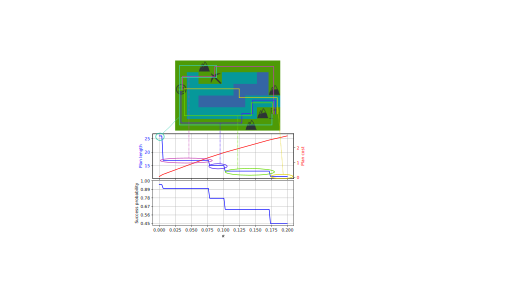
\includegraphics[width=0.9\textwidth]{terrain03alpha-plot}

	\caption{}
	\label{fig:terrain03alpha-plot}. 
\end{figure}

\begin{figure}[p]
	\centering
	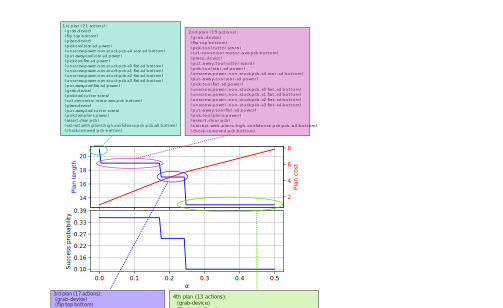
\includegraphics[width=\textwidth]{imagine01alpha}
	\caption{}
	\label{fig:imagine01alpha}. 
\end{figure}

\begin{figure}[p]
	\centering
	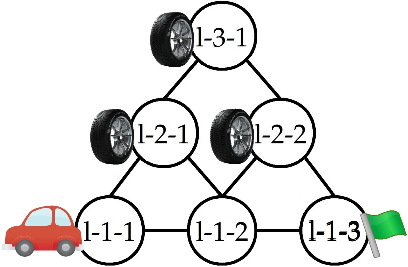
\includegraphics[width=0.5\textwidth]{ttw-p01-crop}
	\caption{}
	\label{fig:ttwmap}. 
\end{figure}

\section{Hindsight Determinization}

\begin{figure}[tbhp]
	\centering
	\begin{subfigure}[b]{0.6\columnwidth}
		\includegraphics[width=\textwidth]{hindsight-wheel-global}
		\caption{}
	\end{subfigure}
	
	\begin{subfigure}[b]{0.8\columnwidth}
		\includegraphics[width=\textwidth]{hindsight-wheel-local}
		\caption{}
	\end{subfigure}
	\caption{
		(a) 
		(b)
	}
	\label{fig:hindsight-wheels}
\end{figure}

\begin{figure}[tbhp]
	\centering
	\begin{subfigure}[b]{0.56\columnwidth}
		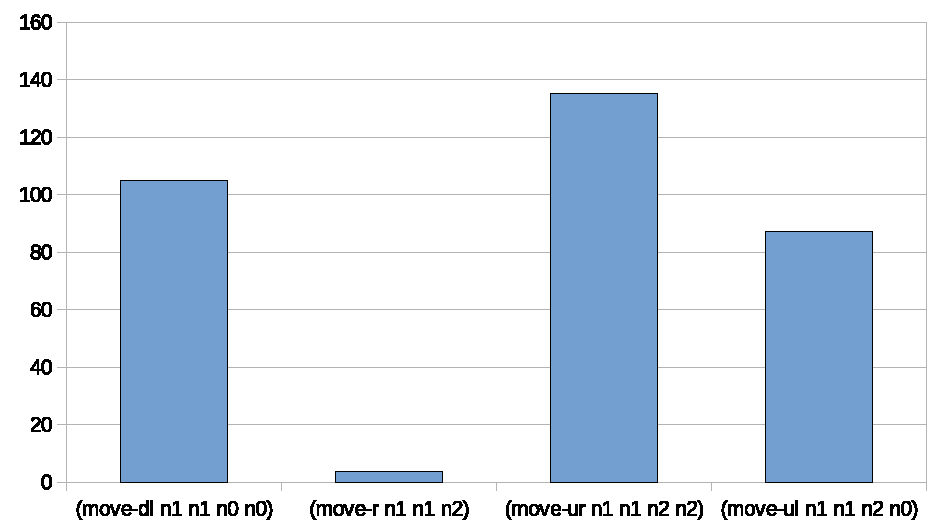
\includegraphics[width=\textwidth]{rectangle-tireworld-hist}
		\caption{}
	\end{subfigure}
	~
	\begin{subfigure}[b]{0.30\columnwidth}
		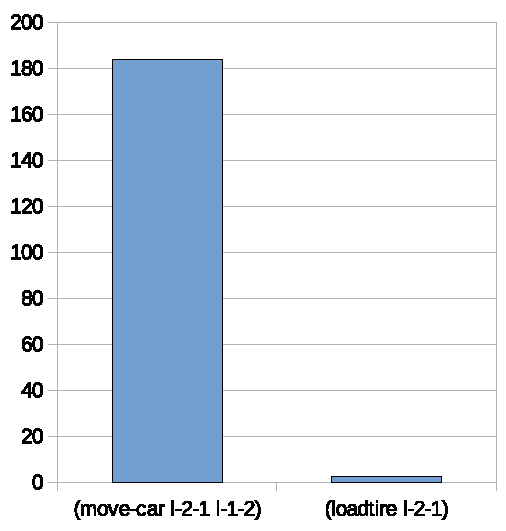
\includegraphics[width=\textwidth]{triangle-tireworld-hist}
		\caption{}
	\end{subfigure}
	\caption{
		(a) 
		(b)
	}
	\label{fig:hindsight-hists}
\end{figure}

\IfEq{\jobname}{\detokenize{root}}{}{\printbibliography}

\end{document}